
很多開發者在學習上一節的內容時,第一反應通常是這樣的:“謝謝!我現在理解了為什麼我的程序很慢,但我必須處理我的數據,不只是理想的32KB,算法就是這樣,包括複雜的數據訪問模式,所以我無能為力。”如果不瞭解如何為需要解決的問題獲得更好的內存性能,那麼這一章就沒有多大意義。本節中,將瞭解可以用來提高內存性能的技術。

\subsubsubsection{4.5.1\hspace{0.2cm}節約內存數據結構}

就內存性能而言,數據結構或數據組織的選擇通常是開發者所做的重要的決策。重要的是要理解能做什麼和不能做什麼。圖4.5和圖4.6展示了內存性能,這裡不能繞過它(嚴格地說,這是99\%的正確。有一些奇異的內存訪問技術,很少會超過這些圖中所示的限制)。但可以在這些圖上選擇與自己程序相對應的點。首先考慮一個簡單的示例。有1M個64位的整數,需要按順序存儲和處理。可以將這些值存儲在數組中,數組的大小將為8MB。根據測試,每個值的訪問時間約為0.6納秒,如圖4.6所示。

%\hspace*{\fill} \\ %插入空行
\begin{center}
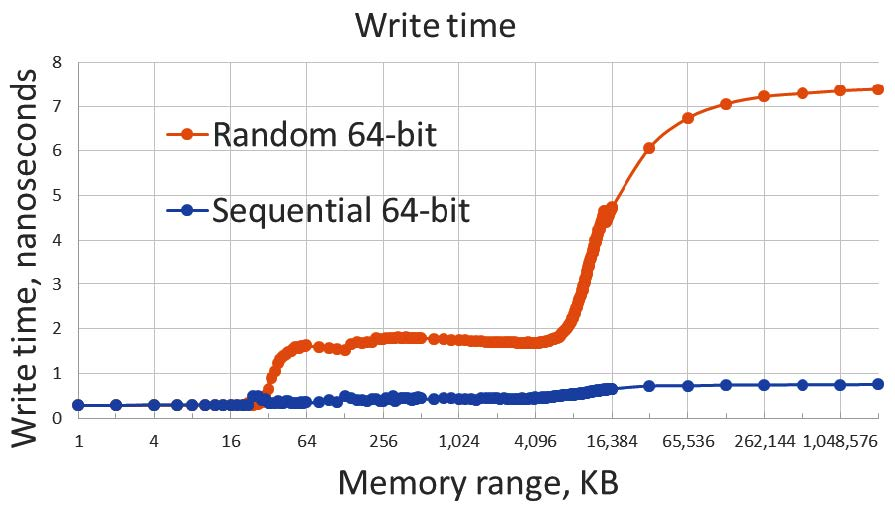
\includegraphics[width=0.9\textwidth]{content/1/chapter4/images/9.jpg}\\
圖4.9 - 寫入數組(A)[隨機]和列表(L)[順序]的時間
\end{center}

首先,可以使用鏈表來存儲。\texttt{std::list}是節點的集合,每個節點都有一個值和兩個指向下一個和上一個節點的指針。因此,整個鏈表使用24MB的內存。此外,每個節點通過對\texttt{operator new}的單獨調用來分配,因此不同的節點可能位於不同的地址,特別是當程序同時進行其他內存分配和回收時。在遍歷這個鏈表時,訪問的地址沒有任何模式,所以要找到這個鏈表的性能點,需要做的就是在曲線上找到對應於隨機內存訪問的24MB內存範圍的點。這使得每個值的訪問比數組中的相同數據慢了5納秒或一個數量級。

這些,前一章已經證明。可以構造一個微基準來比較將數據寫入相同大小的鏈表和數組的區別。以下是數組的基準測試:

\hspace*{\fill} \\ %插入空行
\noindent
\textbf{03\_list\_vector.C}
\begin{lstlisting}[style=styleCXX]
template <class Word>
void BM_write_vector(benchmark::State& state) {
	const size_t size = state.range(0);
	std::vector<Word> c(size);
	Word x = {};
	for (auto _ : state) {
		for (auto it = c.begin(), it0 = c.end(); it !=
		it0;) {
			REPEAT(benchmark::DoNotOptimize(*it++ = x);)
		}
		benchmark::ClobberMemory();
	}
}
BENCHMARK_TEMPLATE1(BM_write_vector, unsigned long)-
>Arg(1<<20);
\end{lstlisting}

將\texttt{std::vector}改為\texttt{std::list}來創建一個基準測試。與之前的基準測試相比,現在是容器中元素的數量已經發生了變化,因此內存大小將取決於元素類型和容器本身,如圖4.6所示。對於1M個元素,結果與預期完全一致:

%\hspace*{\fill} \\ %插入空行
\begin{center}
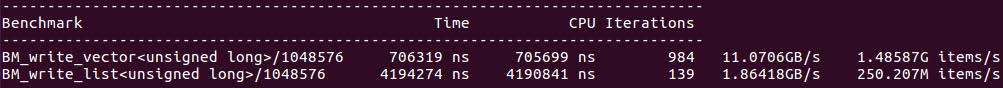
\includegraphics[width=0.9\textwidth]{content/1/chapter4/images/10.jpg}\\
圖4.10 - 鏈表和數組的基準測試結果
\end{center}

為什麼會有人選擇鏈表,而不是數組(或\texttt{std::vector})?最常見的原因是,在創建時不知道有多少數據,並且由於涉及複製,增長\texttt{std::vector}的效率非常低。有幾種方法可以解決這個問題,有時可以預先計算出數據的最終大小,需要對輸入數據進行一次掃描,以確定為結果分配多少空間。如果有效地組織了輸入,那麼可能需要對輸入進行兩次傳遞:第一次是計數,第二次是進行處理。

如果不能提前知道最終的數據大小,可能需要一種更智能的數據結構,將\texttt{vector}的內存與\texttt{list}的調整大小效率結合起來。這可以通過使用塊分配數組來實現:

%\hspace*{\fill} \\ %插入空行
\begin{center}
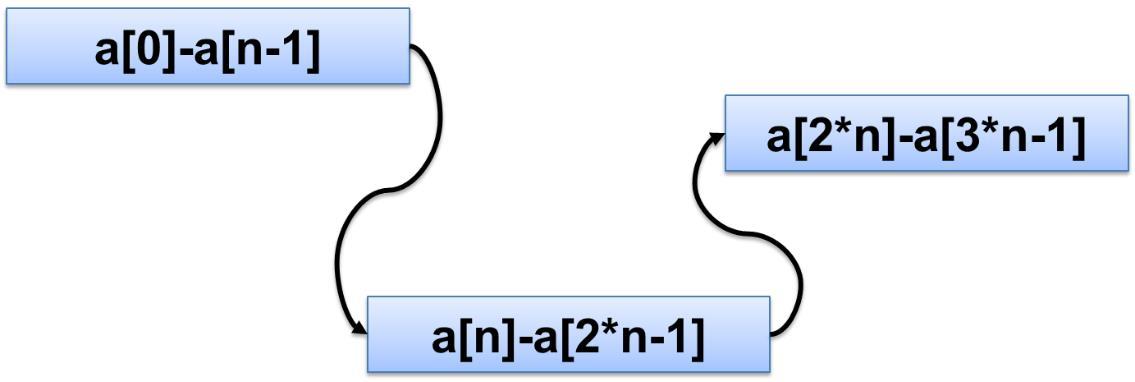
\includegraphics[width=0.6\textwidth]{content/1/chapter4/images/11.jpg}\\
圖4.11 - 塊分配的數組(deque)可以在適當的位置進行增長
\end{center}

這種數據結構以固定數量的塊分配內存,通常小到足以裝入L1緩存(通常在2KB到16KB之間)。每個塊都用作數組,因此每個塊將順序訪問元素,而塊本身在在一個鏈表中。我們需要擴展這個數據結構,只分配一個塊,並將其添加到鏈表中。訪問每個塊的第一個元素很可能會導致緩存丟失,但是當預取檢測到順序訪問的模式時,塊中的其他元素可以高效地訪問。按每個塊中的元素數量平攤,隨機訪問的代價可以變得非常小,數據結構的性能幾乎與數組相同。在STL中,有這樣一個數據結構:\texttt{std::deque}(但大多數STL版本的實現不是特別高效,順序訪問\texttt{deque}通常比訪問相同大小的\texttt{vector}慢一些)。

另一個原因是,鏈表允許在任何點進行快速插入,而不僅僅是在末尾。如果需要,必須使用鏈表或另一個節點分配的容器。這種情況下,最好的解決方案不是選擇一個適合所有需求的數據結構,而是將數據從一個數據結構遷移到另一個數據結構。如果想使用鏈表來存儲數據元素,每次存儲一個,同時保持排序順序,那麼問題來了,我們是否需要在所有元素插入後,對該順序進行排序?還是,需要在構建過程的中間進行幾次排序,而不是一直進行排序?

如果算法中發生了數據訪問模式的改變,那麼改變的數據結構通常對算法有利,即使要付出一些內存複製的代價。可以構造一個鏈表,在添加最後一個元素之後,將其複製到數組中,以加快順序訪問(假設不需要添加更多元素)。我們可以確保數據的某些部分完整,可以將該部分轉換為數組,可能是塊分配數組中的一個或多個,並將可變的數據保留在鏈表或樹的數據結構中。另一方面,如果很少需要按順序處理數據,或者需要按多個順序處理數據,那麼將順序索引與存儲數據區分開保存,通常是最好的解決方案。數據存儲在\texttt{vector}或\texttt{deque}容器中,其順序由按所需順序排序的指針數組保存。由於現在所有的有序數據訪問都是間接的(通過中間指針),很少有這樣訪問的情況下這沒問題;而在大多數情況下,可以按照數據存儲在數組中的順序處理數據。

若是經常訪問一些數據,應該選擇使最優特定訪問模式的數據結構。訪問模式隨著時間的推移而改變,數據結構也應該改變。另一方面,如果不花太多時間訪問數據,那麼從一種數據格式轉換到另一種數據格式的開銷就不合理了。這種情況下,效率低下的數據訪問從一開始就不應該存在。這就引出了下一個問題:如何確定哪些數據訪問效率低,或者說,哪些數據訪問成本高呢?

\subsubsubsection{4.5.2\hspace{0.2cm}分析內存性能}

通常,特定數據結構或數據組織的效率相當高,有一個包含數組或\texttt{vector}的類,並且這個類的接口只允許一種數據訪問模式,即從開始到結束的順序迭代(STL語言中的前向迭代器),那麼可以確定數據可以進行高效地訪問(在內存級別上)。這裡,不能確定算法的效率。若對數組中特定元素的線性搜索非常低效(當然,每次讀取內存都是高效的,但是方法有很多。而且,我們知道更好的方法來組織數據進行搜索)。

僅僅知道哪些數據結構是內存高效的並不夠,還需要知道程序在特定的數據上花費了多少時間。有時,這是不言自明的,特別是對封裝良好的函數。如果有一個函數,從數據文件或時間報告得知其需要大量的時間,並且函數內的代碼不是特別繁重的計算,而是移動大量的數據,那麼更高效地訪問這些數據很可能提升程序整體的性能。

這是一個簡單的例子,因此會首先進行優化。在執行時間上,沒有一個函數或代碼有很大的計算量,但是程序仍然很慢。要是沒有計算量的熱代碼,那通常會有數據的熱代碼。在程序中訪問一個或多個數據結構,在這些數據上花費時間很大,但沒有任何其他函數或循環。傳統的分析會顯示運行時均勻地分佈在整個程序中,優化任何一段代碼都收效甚微。需要某種方法找到那些,低效訪問的數據。

僅靠計時工具很難收集這些信息,但利用硬件事件計數器的分析器可以收集相關信息。大多數CPU都可以計算內存訪問,更確切地說,可以計算緩存命中和未命中。這裡,再次使用\texttt{perf}分析器,通過下面的命令,可以看到L1緩存的使用效率:

\begin{tcblisting}{commandshell={}}
$ perf stat -e \
    cycles,instructions,L1-dcache-load-misses,L1-dcache-loads \
    ./program
\end{tcblisting}

緩存測量計數器不是默認計數器集的一部分,必須顯式指定。可用計數器的集合因CPU而不同,但可以通過運行\texttt{perf list}命令查看。我們的例子中,在讀取數據時測量L1緩存未命中。術語\textbf{dcache}代表\textbf{數據緩存}(data cache,發音為dee-cache)。CPU還有一個單獨的\textbf{指令緩存}或\textbf{icache}(唸作ay-cache),用於從內存中加載指令。

可以使用這個命令行參數,來配置內存基準測試來讀取隨機地址的內存。當內存範圍很小(比如:16KB),整個數組就能放入L1緩存中,幾乎不會出現緩存未命中的情況:

%\hspace*{\fill} \\ %插入空行
\begin{center}
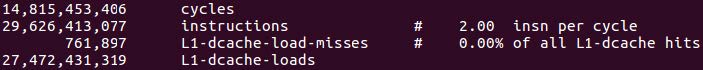
\includegraphics[width=0.9\textwidth]{content/1/chapter4/images/12.jpg}\\
圖4.12 - 測試良好使用L1緩存的程序
\end{center}

將內存大小增加到128MB意味著緩存未命中非常頻繁:

%\hspace*{\fill} \\ %插入空行
\begin{center}
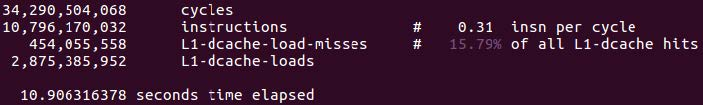
\includegraphics[width=0.9\textwidth]{content/1/chapter4/images/13.jpg}\\
圖4.13 - 測試未良好使用L1緩存的程序
\end{center}

注意,\texttt{perf stat}會收集整個程序的測量值,其中一些內存訪問是緩存高效的,一些不是。想知道哪裡對內存訪問的處理很糟糕,可以使用\texttt{perf record}和\texttt{perf report}獲得詳細的數據信息,如第2章所示(使用了不同的計數器,但是選擇收集數據的過程是相同的)。當然,如果最初的數據沒有檢測到任何熱代碼,緩存數據也會顯示同樣的結果。代碼中的許多位置,緩存未命中的比例都很大。每個位置對總體執行時間沒什麼貢獻,但這會累積。現在,這些代碼位置中的許多都有一個共同點,對內存進行操作。若有幾十個不同的函數,總共佔15\%的緩存未命中率,但都在同一個鏈表上運行,那麼這個鏈表就是有問題的數據結構,必須以其他方式組織數據。

現在已經瞭解瞭如何檢測和識別那些低效的內存訪問模式,和會對性能產生負面影響的數據結構,以及相關的替代方案,但可供選擇的數據結構通常沒有相同的特性或性能。如果從數據結構的整個生命週期來看,必須在任意位置插入元素,則不能用\texttt{vector}替換\texttt{list}。若不是數據結構,而是算法本身調用了低效率的內存訪問,則需要改變算法。

\subsubsubsection{4.5.3\hspace{0.2cm}優化內存性能的算法}

算法的內存性能會經常忽視。選擇算法通常根據其\textbf{算法性能}或執行的操作或步驟的數量進行的,內存優化通常需要反直覺的選擇。做更多的工作,甚至不必要的工作,以提高內存性能,這裡是用一些計算來換取更快的內存操作。因為內存操作很慢,所以要做的工作也很多。

更快地使用內存的方法是使用更少的內存,這種方法通常會需要重新計算一些本可以存儲和從內存中檢索的值。最壞的情況是,如果檢索結果需要隨機訪問,讀取每個值需要幾納秒(在我們這是7納秒)。重新計算這個值所花費的時間比這要少,而將7納秒轉換為CPU可以執行的操作數是相當長的時間,那麼最好不存儲這些值。這是傳統的空間與內存的交換。

這種優化有一個有趣的變式。在特定時間內使用更少的內存,而不是簡單地使用更少的內存。這裡是想將當前工作的數據集放入緩存中,比如L2緩存,並在移動到數據的下一部分之前對它進行儘可能多的處理。將新數據集插入到緩存中會導致內存地址的緩存未命中,最好接受這一次緩存未命中,然後在一段時間內有效地操作數據。而非一次處理所有數據,並在每次需要此數據元素時,會有緩存未命中的風險。

這一章,將通過更多的內存訪問來保存一些其他的內存訪問。這裡是希望減少緩慢的、隨機的訪問次數,但增加了快速的、連續的訪問次數。由於順序內存流比隨機訪問快一個數量級,還有很多額外的工作,以減少緩慢的內存訪問。

演示需要一個更詳細的示例。假設有一組數據記錄,比如字符串,程序需要對其中一些記錄進行一些更改。然後得到另一組修改後的數據,以此類推。每個集合將對某些記錄進行更改,而其他記錄保持不變。通常,這些變化會改變記錄的大小及其內容。在每個集合中更改的記錄子集是完全隨機和不可預測的。以下是一張演示圖表:

%\hspace*{\fill} \\ %插入空行
\begin{center}
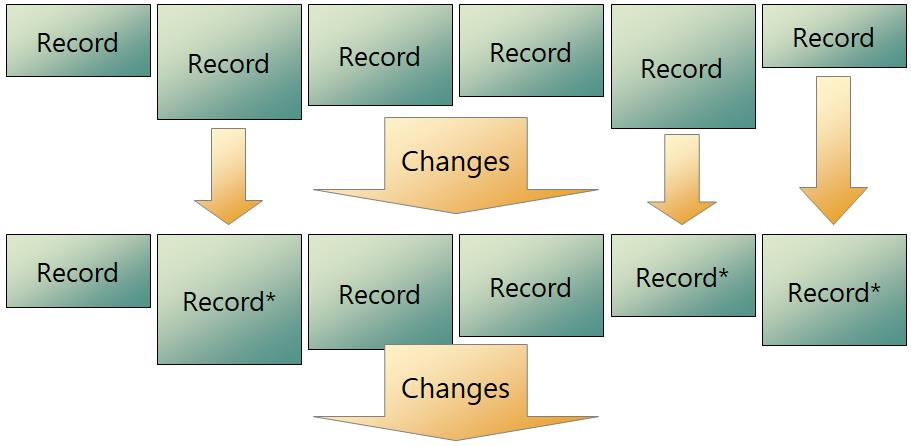
\includegraphics[width=0.7\textwidth]{content/1/chapter4/images/14.jpg}\\
圖4.14 - 記錄編輯問題。在變更集中,由*標記編輯過的記錄,其餘的保持不變
\end{center}

解決這個問題最簡單的方法是將記錄存儲在它們自己的內存中,並將它們組織在某種數據結構中,允許新記錄的替換(因為新記錄的大小通常不同,需要重新為舊記錄進行分配),數據結構可以是樹(在C++中設置)或鏈表。為了讓這個例子更加具體,這裡使用字符串作為記錄,還必須說明更改集的指定方式。它沒有指向需要更改的特定記錄,但對於每個記錄,都可以對其進行更改。這種字符串更改集的最簡單示例是查找和替換。這裡,可以簡單描述一下實現:

\begin{lstlisting}[style=styleCXX]
std::list<std::string> data;
… initialize the records …
for (auto it = data.begin(), it0 = --data.end(), it1 = it;
true; it = it1) {
	it1 = it;
	++it1;
	const bool done = it == it0;
	if (must_change(*it)) {
		std::string new_str = change(*it);
		data.insert(it, new_str);
		data.erase(it);
	}
	if (done) break;
}
\end{lstlisting}

每個更改集中,都遍歷整個記錄集合,確定是否需要更改記錄。如果需要,就這進行變更(更改集隱藏在函數\texttt{must\_change()}和\texttt{change()}中)。代碼只顯示一個更改集,因此需要循環多次運行。

這個算法的缺點是使用了鏈表,更糟的是一直在內存中移動字符串。對新字符串的訪問會出現緩存未命中。如果字符串非常長,那麼初始的緩存未命中就不重要了,其餘的字符串可以使用順序訪問快速讀取。結果與前面的塊分配數組相似,而且內存性能良好。如果字符串很短,那麼整個字符串很可能在一次加載操作中讀取,並且每次加載都是在一個隨機地址上進行。

整個算法只在隨機地址處做加載和存儲,這是訪問內存最糟糕的方法。那我們能做什麼呢?不能將字符串存儲在巨大的數組中。如果數組中間的字符串需要增長,那麼內存從哪裡來?該字符串後面是另一個字符串,所以這裡已經沒有增長的空間了。

想出的替代方案,需要進行範式轉換。按字面意思執行所需操作的算法也對內存組織施加了限制。更改記錄需要將它們移動到內存中,而且希望能夠在不影響其他東西的情況下更改記錄,所以就不能避免內存中記錄的隨機分佈。必須從側面來看待這個問題,從限制開始。按順序訪問所有的記錄,在這個約束下,我們能做什麼?可以很快地讀取所有記錄。可以決定記錄是否更改,這一步和之前一樣。如果記錄必須增加,該怎麼辦?必須把它移到別的地方去,這些記錄要按照先後順序分配。然後,前一個記錄和下一個記錄也必須移動,因此它們在新記錄之前和之後都保持存儲狀態。這是替代算法的關鍵:所有記錄都隨著每個變更集移動,無論它們是否更改。可以將所有記錄存儲在一個巨大的連續緩衝區中(假設已知總記錄大小的上限):

%\hspace*{\fill} \\ %插入空行
\begin{center}
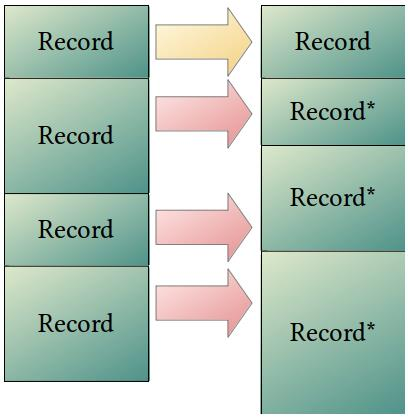
\includegraphics[width=0.25\textwidth]{content/1/chapter4/images/15.jpg}\\
圖4.15 - 按順序處理所有記錄
\end{center}

算法要求在複製過程中分配大小相等的第二個緩衝區,因此內存消耗峰值是數據大小的兩倍:

\begin{lstlisting}[style=styleCXX]
char* buffer = get_huge_buffer();
… initialize N records …
char* new_buffer = get_huge_buffer();
const char* s = buffer;
char* s1 = new_buffer;
for (size_t i = 0; i < N; ++i) {
	if (must_change(s)) {
		s1 = change(s, s1);
	} else {
		const size_t ls = strlen(s) + 1;
		memcpy(s1, s, ls);
		s1 += ls;
	}
	s += ls;
}
release(buffer);
buffer = new_buffer;
\end{lstlisting}

每個更改集中,將每個字符串(記錄)從舊緩衝區複製到新緩衝區。如果需要更改記錄,則將新版本寫入新的緩衝區;否則,將原始版本複製。對每個新的更改集,創建一個新的緩衝區,並在操作結束時釋放舊的緩衝區(實現需要避免重複調用分配和釋放內存,並簡單地交換兩個緩衝區)。

這種實現的缺點是使用巨大的緩衝區。必須確定緩衝區的大小,以便為可能遇到的最大記錄分配足夠的內存。峰值內存的大小也令人擔憂,可以通過將這種方法與可增長數組數據結構相結合來解決這個問題。可以將記錄存儲在一系列大小固定的塊中,而不是分配在一個連續的緩衝區中:

%\hspace*{\fill} \\ %插入空行
\begin{center}
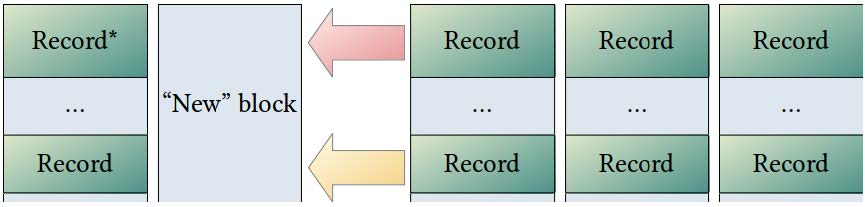
\includegraphics[width=0.9\textwidth]{content/1/chapter4/images/16.jpg}\\
圖4.16 - 使用塊緩衝區進行編輯
\end{center}

為了簡化圖表,我們繪製了相同大小的所有記錄,但是這個限制是不必要的。記錄可以跨越多個塊(將這些塊視為一個連續的字節序列,僅此而已)。當編輯時,需要為已編輯的記錄分配一個新塊。編輯完成後,可以釋放包含舊記錄的塊(或多個塊),從而不必等待讀取整個緩衝區。甚至,可以將最近釋放的塊放到空塊鏈表中,而不是返回操作系統。即將編輯下一個記錄,將需要一個空的新塊作為結果。剛好,這是塊用來包含我們編輯的最後一個記錄。它位於最近發佈的塊鏈表的頭部,最重要的是,這個塊是訪問的最後一塊內存,所以它可能仍然在緩存中!

乍一看,這個算法似乎非常糟糕,每次都要複製所有的記錄。仔細地分析這兩種算法。首先,讀取的數量相同:兩種算法都必須讀取每個字符串,以確定是否更改。第二種算法在性能上領先:在一次連續掃描中讀取所有數據,而第一種算法則在內存中跳躍。如果編輯該字符串,那麼兩個算法都必須向新的內存區域寫入一個新的字符串。由於順序內存訪問模式(同樣,不需要為每個字符串執行內存分配),第二種算法提前出現了。當字符串未編輯時,就需要進行權衡。第一個算法什麼都不做,第二個做了一個拷貝。

通過這種分析,可以為每個算法定義好的和壞的情況。如果字符串很短,並且在更改集中更改了大部分字符串,則順序訪問算法勝出。如果字符串很長或者很少改變字符串,隨機訪問算法就會獲勝。然而,確定什麼是長、多少是大比例的唯一方法就是測試。

這裡,不一定意味著必須編寫完整程序的兩個版本進行測試。通常,可以對簡化數據進行操作的小型模擬程序中模擬特定的行為。只需要知道記錄的大致大小,有多少條更改記錄,並且需要對單個記錄進行更改的代碼,這樣就可以測試內存訪問對性能的影響(如果每次更改影響都非常大,那麼讀取或寫入記錄所花費的時間就無關緊要了)。可以對這樣的模擬或原型實現進行近似測試,並做出正確的設計決策。

實際中,順序字符串複製算法值得一試麼?我們已經完成了使用正則表達式模式編輯中等長度字符串(128字節)的測試。所有字符串的99\%都在每個更改集中進行編輯,順序算法的速度大約是隨機算法的4倍(結果在某種程度上是特定於機器的,因此必須在與預期使用的硬件相似的硬件上進行測試)。編輯了50\%的記錄時,順序訪問仍然更快,但是隻有12\%的性能提升(這可能是在不同的CPU模型和內存類型的變化範圍內,所以稱之為平局)。更令人驚訝的是,如果只更改了1\%的記錄,那麼這兩種算法的速度幾乎是成正比的,不進行隨機讀取所節省的時間將用來彌補完全不必要的複製。

改動較長的字符串,隨機訪問算法輕鬆獲勝。如果改變很少的字符串,而且對於非常長的字符串,即使所有的字符串都改變,也是平局。兩種算法都依次讀取和寫入所有字符串(對長字符串開始的隨機訪問增加的時間可以忽略)。

現在我們已經掌握了應用程序所需的所有算法。性能設計通常是這樣的:確定性能問題的根源,並想出消除問題的方法,但代價是要做其他更多事情,然後必須建立一個測試,讓我們能夠確定這個方法是否真的有效。

本章的最後,將展示一個完全不同的“使用方式”,由緩存和其他硬件提供的性能改進。




























